\section{Generalities}
All primary displays use electrical power from the secondary AC bus.
The displays are turned on when switching the main mode selector
(\cockpitref{fig:left-panel}{item:main-mode}) from BER/PRE to NAV.

Displays require some preheating before being functional:
\begin{itemize}
  \item The HUD turns on at the earliest 30 seconds after AC power is available.
  \item The CI turns on at the earliest 30 seconds after switching to mode NAV.
\end{itemize}

\section{Head Up Display (HUD)}
\subsection{Overview}
\begin{figure}[!ht]
  \centering
  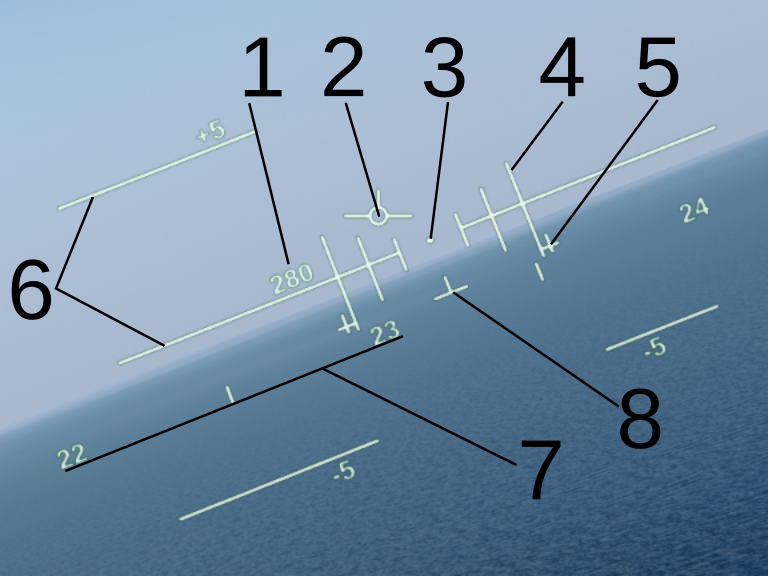
\includegraphics[width=0.6\textwidth]{images/displays/ajs-hud-general.png}

  \begin{multicols}{2}
    \begin{enumerate}[nosep]
      \item \label{item:digalt} Digital altitude
      \item \label{item:fpv} Flight path vector
      \item \label{item:refpt} Reference point
      \item \label{item:alt} Altitude bars
      \item \label{item:refbars} Reference bars and radar altitude index
      \item \label{item:horizon} Artificial horizon and pitch lines
      \item \label{item:heading} Heading scale
      \item \label{item:timeline} Time / distance scale
    \end{enumerate}
  \end{multicols}

  \caption{HUD overview}
  \label{fig:hud}
\end{figure}

\subsection{Controls}
HUD brightness is adjusted with knob \cockpitref{fig:front-panel}{item:hud-bright}.
The following two switches located on the lower right of the HUD
(\cockpitref{fig:front-panel}{item:hud-switch}) affect the HUD presentation.

\paragraph{SLAV SI (SLV HUD)}
In navigation mode, this switch enables a decluttered low-altitude mode when
in position T (ON), see \cref{sec:hud-declutter}.

During optical landing, if in position T (ON), the HUD reference point will
be aligned with the flight path vector, instead of indicating runway heading.

\paragraph{HÖJD CI SI (ALT DISP)}
When in position RHM (RAD), the radar altimeter is used to compute a ground
corrected altitude, which is displayed on the HUD.
Otherwise, displayed altitude is the same as on the main altimeter.

The switch automatically goes back to position LD (BAR) at altitude >2450m
and during landing final phase.

\subsection{Navigation Mode}
\paragraph{Artificial Horizon (\cockpitref{fig:hud}{item:horizon})}
The artificial horizon and the +5 and -5 degrees pitch lines provide an attitude reference.
The HUD does not have a full pitch scale, only the horizon and the +5 and -5 degrees lines.

Horizontally, the artificial horizon is pointing towards the current destination,
indicated by the reference point (\cockpitref{fig:hud}{item:refpt}).

\paragraph{Flight Path Vector (\cockpitref{fig:hud}{item:fpv})}
The FPV marker indicates the aircraft path direction relative to the ground.
When on the horizon, the aircraft is in level flight.
When covering the reference point, the aircraft track coincides with the destination.

\paragraph{Digital Altitude (\cockpitref{fig:hud}{item:digalt})}
Displays the aircraft altitude.
Below 1km the altitude is displayed in meters with a precision of 10m.
Above 1km the altitude is displayed in kilometers with a precision of 100m.
Above 10km, the digital altitude cycles back to 0,
thus 1500m and 11500m are both displayed as `1,5'.
Negative altitude up to -90m can be displayed.

\paragraph{Altitude Bars (\cockpitref{fig:hud}{item:alt})}
The 6 altitude bars indicate the aircraft altitude relative to the reference altitude
(also called commanded altitude).

The top of the bars represents the reference altitude,
and the bottom of the bars represent ground level (to be exact, indicated altitude 0m).
The aircraft altitude is indicated by the horizon line.
Thus, if the top of the bars is aligned with the horizon, the aircraft is at the commanded altitude,
and if the bottom of the bars is aligned with the horizon, the aircraft is at ground level.

One can imagine the top, resp.\ bottom of the bars as forming a horizontal
plane in a perspective drawing, located at reference, resp.\ ground altitude.
In this perspective drawing, the vanishing point is the reference point.

If the reference altitude is higher than 500m,
the bottom of the bars represents the reference altitude minus 500m instead of ground level.

\subparagraph{Reference Altitude}
The reference altitude displayed by the altitude bars is set as follows.
\begin{itemize}[noitemsep]
  \item During takeoff, reference altitude is fixed at 500m.
  \item During flight, the reference button (keybinding \keys{\shift+R}) 
    sets it to the current altitude.
  \item If autopilot altitude hold mode is active,
    the reference altitude is the autopilot altitude.
  \item When entering landing mode, reference altitude is set to 500m.
    It can still be modified with the reference button or by engaging autopilot altitude hold.
\end{itemize}

If the difference between reference altitude and current altitude is too large,
the displayed reference altitude will differ from the actual reference altitude.

\subparagraph{Reference Altitude Bars (\cockpitref{fig:hud}{item:refbars})}
The reference altitude bars are located just next to the outer altitude bars.
The length of the reference altitude bars varies to indicate reference altitude:
if the length of the outer altitude bars (which is fixed to 3\textdegree{})
represents the reference altitude, then the length of the reference altitude bars represents 100m.

For instance, in \cref{fig:hud}, the length of the reference altitude bars is
0.6\textdegree{}, i.e.\ 1/5 of the outer altitude bars.
Thus 100m is 1/5 of the reference altitude, i.e.\ the reference altitude is 500m.

At reference altitudes higher than 500m, the reference bars are hidden.

\subparagraph{Radar Altitude Index (\cockpitref{fig:hud}{item:refbars})}
When available, radar altitude is indicated by a horizontal index on the outer altitude bars,
which can be read on the outer altitude bars or the reference altitude bars.

When the index is at the bottom of the altitude bars,
radar altitude and indicated altitude coincide,
which can be used to calibrate the altimeter in flight.
However this method is only accurate when reference altitude is at most 500m
(reference altitude bars are displayed).

\paragraph{Heading Scale (\cockpitref{fig:hud}{item:heading})}
Indicates current heading.
Every 10\textdegree{} is indicated by a number,
and every 5\textdegree{} between them by a vertical mark.
The scale is 1:1, i.e.\ the bearing of a world object can be read directly on the scale.

\paragraph{Time and Distance Scale (\cockpitref{fig:hud}{item:timeline})}
Indicate time or distance to an event or waypoint.
The line shrinks and grows horizontally around the center to indicate time or distance to the event.
A vertical center mark, and in some modes two side marks, represent the events.
\begin{itemize}
  \item During takeoff roll, the line grows to indicate aircraft speed.
    The side marks indicate recommended rotation speed.
  \item In navigation mode, the line represents time to the next waypoint.
    It appears 60 seconds before the waypoint, and shrinks until reaching the waypoint.
  \item In cannon or rocket aiming modes, the line indicates distance to target,
    and the side marks indicate minimum firing distance.
\end{itemize}

\subsection{Low Altitude Declutter}
\label{sec:hud-declutter}
If the switch SLAV SI is in position T (TILL), a decluttered HUD is displayed at altitude <100m.
In this decluttered mode, only the flight path vector,
artificial horizon, and digital altitude are displayed.
Pressing the reference button (keybinding \keys{\shift+R})
in decluttered mode toggles the heading scale.

\subsection{Takeoff Mod}
Takeoff mode is enabled is enabled when the nose gear is compressed,
provided the master mode selector is not in mode LANDING.

During takeoff, the FPV is fixed 10\textdegree{} below the aircraft forward axis,
and the FPV marker vertical fin is hidden.
The artificial horizon reference point is aligned with the aircraft forward axis.
Time line and heading scale are fixed 10\textdegree{} below the horizon.
The time line indicates airspeed, with the side markers corresponding to rotation speed.

When the rotation angle reaches 5\textdegree{},
the time line is hidden and the heading scale moves to its normal position.

Takeoff mode stops when the airspeed exceeds M 0.35,
or when the flight path angle is at least 3\textdegree{} up,
or at landing gear retraction.

\subsection{Landing Mode}
\begin{figure}[!ht]
  \centering
  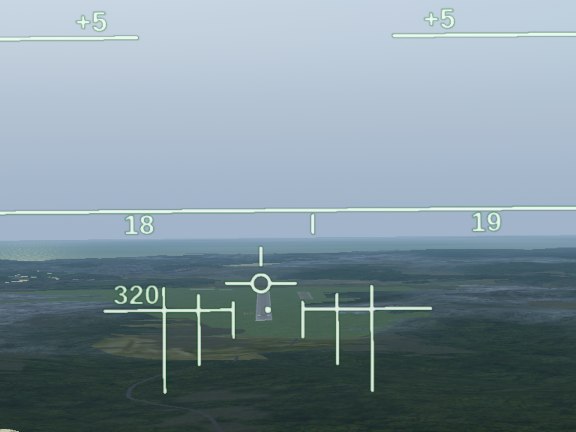
\includegraphics[width=0.5\textwidth]{images/displays/ajs-hud-landing.png}
  \caption{HUD during final}
  \label{fig:hud-landing}
\end{figure}

In landing mode, the HUD changes when starting the final.
The -5\textdegree{} pitch lines are removed,
and a glideslope line is added 2.86\textdegree{} below the horizon
(corresponding to a slope of 5\%).
Altitude bars and digital altitude are moved from the horizon to the glideslope line,
and the heading scale is moved under the horizon.

\paragraph{Speed / AoA Indicator}
In landing mode, the vertical fin (`tail') of the flight path vector symbol
moves vertically to indicate deviation from the target speed or angle of attack.

The speed is correct when the bottom of the tail is on the FPV circle
(default position in navigation mode).
If the tail is higher than the circle, the aircraft speed is too high.
If the tail is lower (inside the circle), the aircraft speed is too low.

While the landing gear is up, the target speed is 550km/h.
Once the landing gear is down and locked, the target angle of attack is 12\textdegree{}.
If the $\alpha 15,5\degree$ button
(\cockpitref{fig:front-panel}{item:autothrottle-lights}) is pressed (light lit),
the target angle of attack is 15.5\textdegree{} instead.

When the landing gear is down, the fin will blink if the angle of attack is critically high.

\paragraph{ILS Guidance}
If ILS guidance is used, the reference point indicates the heading to follow to align with the localizer,
and the altitude bars indicate ILS glideslope deviation:
if the top of the bars is above, resp.\ below the glideslope line,
the aircraft is below, resp.\ above the ILS glideslope.

If ILS is not used (optical landing mode),
the reference point indicates runway heading and the altitude bars are hidden.

\paragraph{Touchdown}
Below 30m, the HUD switches to optical landing display (ILS indications disappear).
Below 15m radar altitude, the HUD switches to flare mode.
The glideslope line moves up to indicate the descent angle
which gives a vertical speed of 2.96m/s, the maximum for touchdown.
If radar altitude is unavailable, transition to flare mode occurs at 30m.

\subsection{Tactical Information}
Some weapons have specific combat HUD presentations (aiming mode),
enabled by switching to ANF/CBT mode or arming the weapon.
See \cref{chap:weapons} for details.
